\documentclass[11pt]{article}
\usepackage{fullpage}
\usepackage{graphics,epsfig,color}
\usepackage{wrapfig}
\usepackage{times}
\usepackage{setspace}
\usepackage{amsmath,amsthm,amssymb}
\usepackage{url}
\usepackage{fancyhdr}
\usepackage{enumitem}
\pagestyle{fancy}


\newtheorem{theorem}{Theorem}[section]
\newtheorem{corollary}{Corollary}[section]
\newtheorem{lemma}{Lemma}[section]
\newtheorem{problem}{Problem}
\newtheorem{definition}{Definition}[section]
\newtheorem{observation}{Observation}[section]
\newtheorem{example}{Example}[section]
\newtheorem{openproblem}{Open Problem}[section]
\newtheorem{fact}{Fact}[section]

\newcommand{\qedsymb}{\hfill{\rule{2mm}{2mm}}}
\newenvironment{proofsketch}
{
	\begin{trivlist}
	\item[\hspace{\labelsep}{\noindent Proof Sketch: }]
}{\qedsymb\end{trivlist}}



%the following few lines until usepackage{algorithm2e} is to avoid the
%conflicts of algorithm2e with other packages.
\makeatletter
\newif\if@restonecol
\makeatother
\let\algorithm\relax
\let\endalgorithm\relax
\usepackage[ruled,vlined,linesnumbered]{algorithm2e}

\newcommand{\remove}[1]{}



%--------------------------------


\begin{document}

	\renewcommand{\headrulewidth}{0.4pt}
	\setlength{\headheight}{38.0pt}
	\fancyhead[L]{\bf CSCD320 Homework 9, Winter 2012, 
	Eastern Washington University. Cheney, Washington. \\
	\bigskip Name: Eric Fode\hspace{40mm}EWU ID:00530214}

	\noindent{\bf Solution for Problem 1}\\
		In this case no more then the first node will have to be explored to find the shortest path.\\
		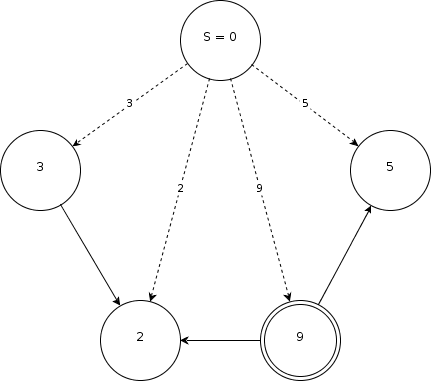
\includegraphics[scale=.5]{D1.png}\\	
	\newpage
	\noindent{\bf Solution for Problem 2}\\
		Three sets of edge relaxation will be required to find the optimum paths.\\
		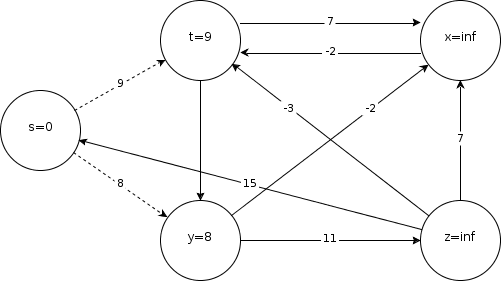
\includegraphics[scale=.5]{BF1.png}\\
		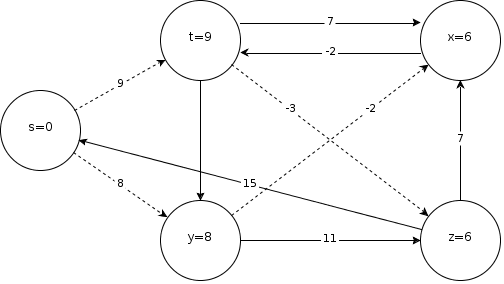
\includegraphics[scale=.5]{BF2.png}\\
		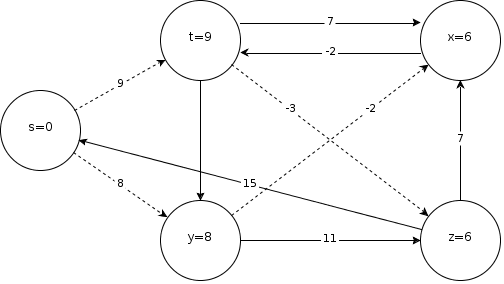
\includegraphics[scale=.5]{BF2.png}\\
	\bigskip
	\noindent{\bf Solution to problem 3}\\	
		Use Warshall's algorithm.
		\begin{enumerate}
			\item Copy the adjacency matrix into another matrix called path.
			\item Find in path every for every vertex the incoming and outgoing edges.
			\item For every pair of edges associated with a vertex that is found put a 1 in the path matrix.
			\item The transitive closure is trivial to extract from the path matrix.
		\end{enumerate}
\end{document}